\section{Reflections}
\label{reflections_section}

This assessment looks like a complete failure.
While some of our models trained better than others, none of the results in \appendixA{} are even close to not being nonsensical.

Why is sequence analysis so hard? These results provide a good clue.
While different metrics from their embeddings tell us that some of them should be better than others, there is simply no intuition on what is wrong, or what could improve.

\begin{figure}[h]
	\begin{subfigure}[][265pt][t]{.48\textwidth}
		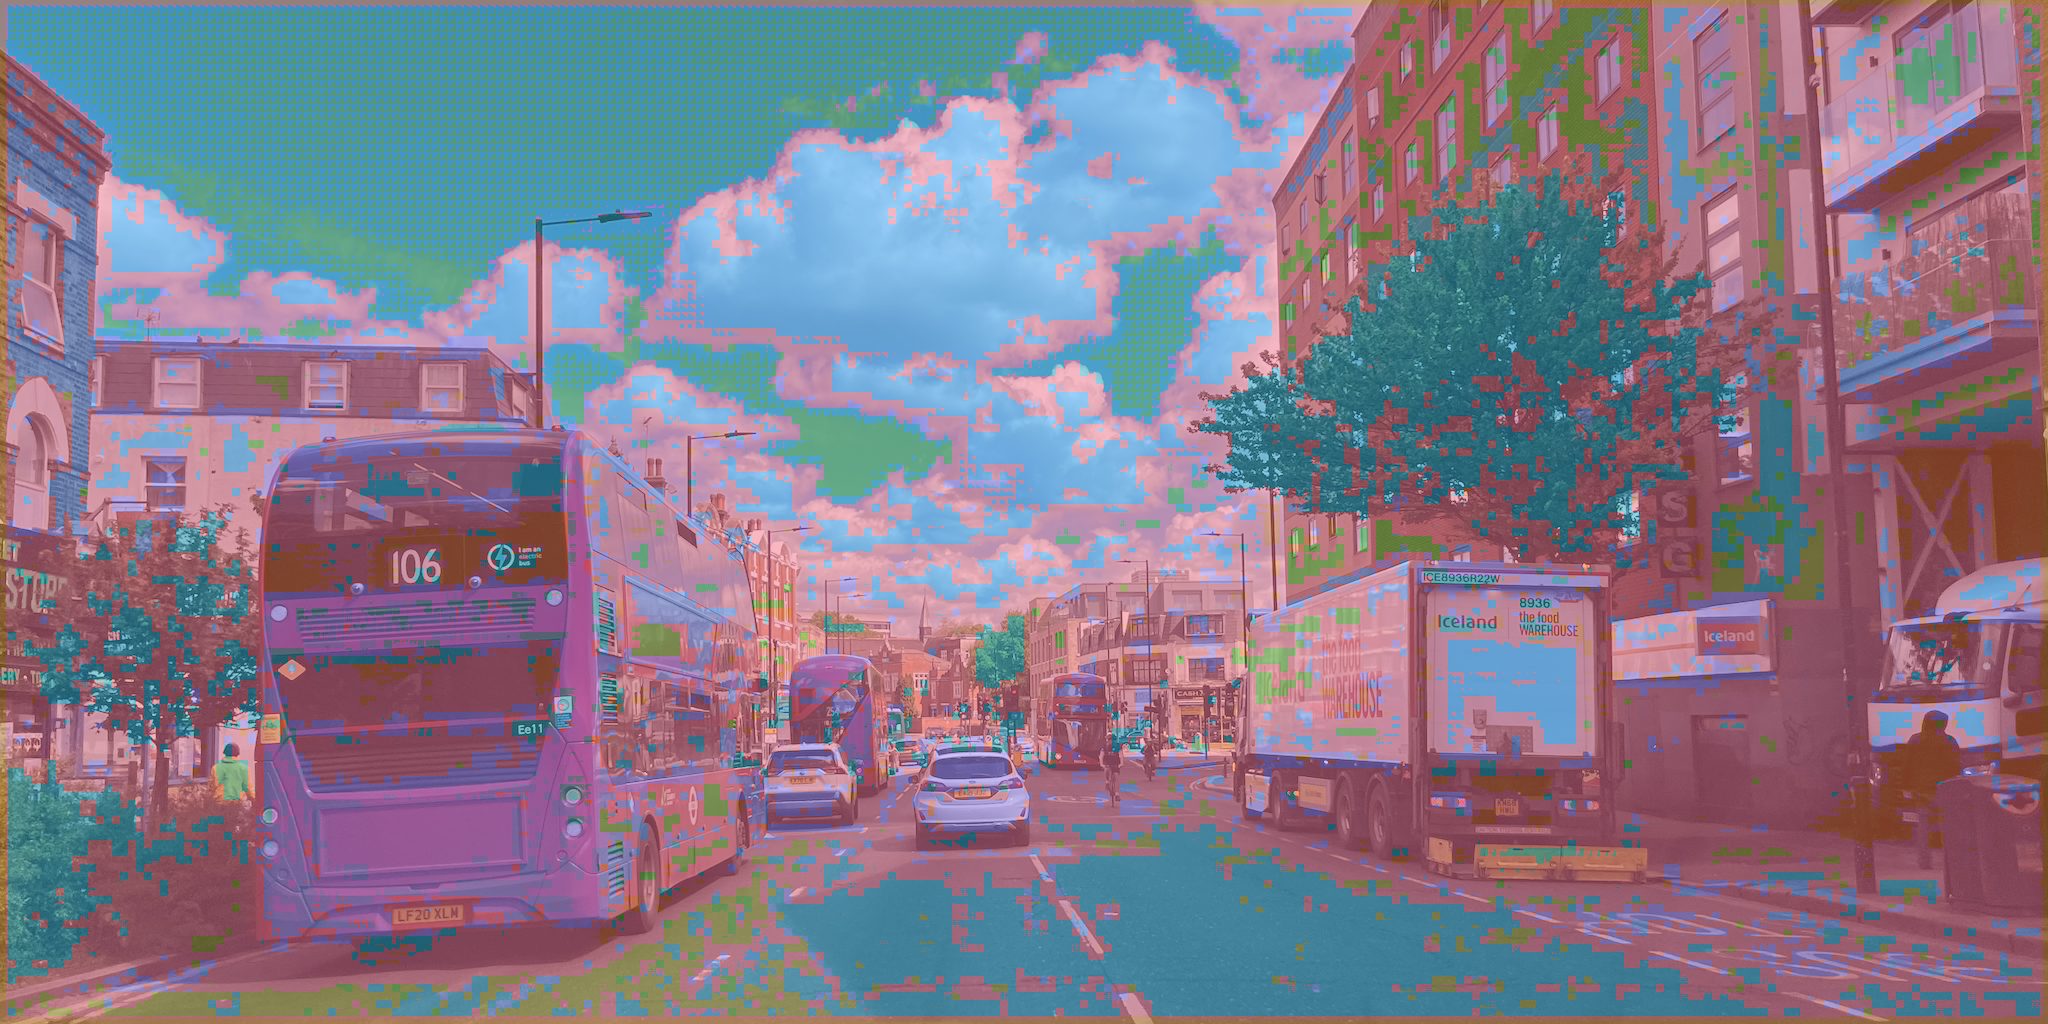
\includegraphics[width=\textwidth]{bad_convolutional_result.png}
		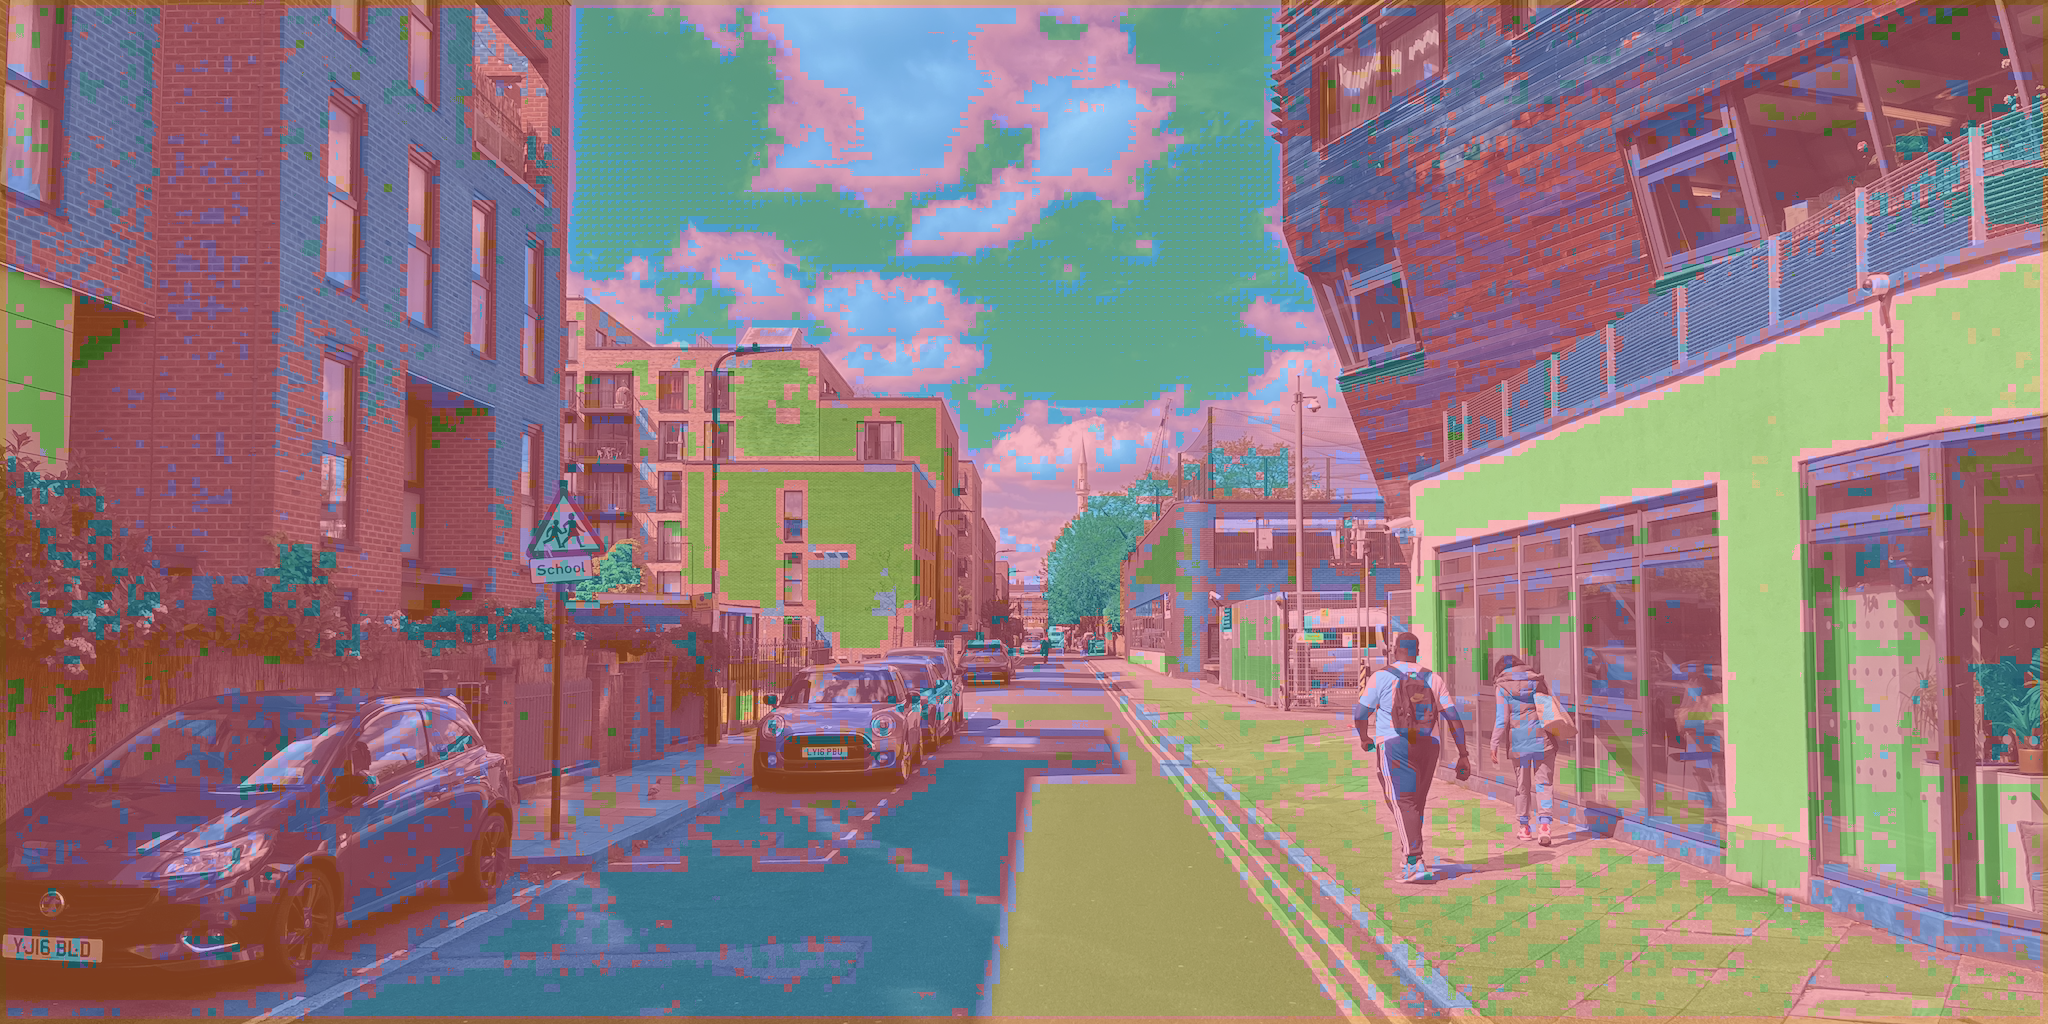
\includegraphics[width=\textwidth]{bad_convolutional_result_2.png}
		\caption{Examples of bad results in an Image Segmentation problem. The areas are pixelated, so we likely need to try a larger kernel size of lower resolutions, and the red bus isn't registered as a vehicle, so we likely need to use different training data. Many more conclusions can be had from this data.} 
	\end{subfigure}\hfill{}%
	\begin{subfigure}[][265pt][t]{.48\textwidth}
		\triplebox{cnn chelsea claimed first silverware english domestic season jose mourinho first trophy second spell charge 2 0 win tottenham hotspur wembley sunday. deflected efforts either side halftime chelsea captain john terry leading scorer diego costa dashed tottenham hopes london league cup final. chelsea suffered chastening christmas defeat opposition english premier league harry kane starring promising young english striker kept largely quiet showpiece occasion. first half saw tottenham edge possession carry attacking threat dane christian eriksen free kick rattling chelsea crossbar. chances either side open play short supply free kick chelsea went ahead break.ian delivery right brushed danny rose head fell invitingly terry whose shot went net taking deflection eric dier. tottenham might felt hard done sense injustice would deepened 56 minutes cesc fabregas found costa left firm strike took another wicked deflection time walker credited goal leave goalkeeper hugooris chance. seemed take sting tottenham challenge although [\dots{}]}{new clinton english premier title title. chelsea mourinho chelsea beat chelsea hotspur. 0.. chelsea terry says chad david game. chelsea chelsea chelsea 2 1 win win london win...l. chelsea chelsea chelsea chelsea chelsea chelsea chelsea chelsea chelsea chelsea chelsea chelsea chelsea chelsea chelsea chelsea chelsea chelsea chelsea chelsea chelsea chelsea chelsea chelsea chelsea chelsea chelsea chelsea chelsea chelsea chelsea chelsea chelsea chelsea chelsea chelsea chelsea chelsea chelsea chelsea}{chelsea wins english league cup wembley. jose mourinho team beats tottenham hotspur 2 0 wembley. john terry kyle walker goal chelsea. man city loses 2 1 liverpool miss chance close chelsea top epl.}

		\caption{A bad result in text summarisation from our own BERTFormer model. There's no useful information to be gathered from here.}
	\end{subfigure}
	\caption{Comparing examples in image analysis with sequence analysis yields one of the reasons why the latter is so difficult: bad results provide no useful information.}
\end{figure}

When looking at the literature at existing examples of models that \emph{do} succeed in news summarisation, they create models that are considerably more complex than the ones in this assessment.

BART\cite{bart_model}, created by the team currently formerly known as Facebook AI, uses a deionising autoencoder finishing with GPT.
While the model is not particularly large, it seems that the noise in the input functions improves the results.
PEGASUS\cite{pegasus_model}, created by engineers at the team formerly known as Google Brain (how quickly things change in the tech world) uses a gap-sentence pre-training which is able to generalise masking to better data.

These two models, among others, present avenues to improve our current models.
Most importantly, they trained with massive amounts of data that weren't available to us due to time and technical reasons.

However, here are some areas where we'd like to continue experimenting.
\begin{description}[style=nextline,noitemsep]
	\item[Embedding Size]
		In retrospect, this was a good area to add to the parameter sweep in \cref{param_sweep_section}.
		It's possible that using only 512 dimensions in the embedding was the reason for the bad performance of our models.
	\item[TF and IDF tokens in the period token]
		While keeping the period token `\textbf{.}' was necessary for our report, calculating TF and IDF tokens for it in the enhanced models does not make sense caused it to become disproportionately important throughout the dataset as it was by far the most common token.
		These metrics should be calculated ignoring this token.
		Alternatively, the end-of-sequence token could be employed to mark sentence boundaries, which might offer a more effective solution.
	\item[Novel uses of masking]
		Similar to how PEGASUS uses Gap-Sentence Generation masking\cite{pegasus_model}, we can train a model to generate missing sentences from a document, mimicking the summarisation task.
		This masking selects ``important'' sentences during training on each input source, which are later masked in the document and the model trained in prediction.
		This works well for summarisation, since it focuses on reconstructing important sentences.
	\item[Non-novel uses of cosine similarity score and loss]
		Cosine Similarity Loss and Scores, introduced in \cref{cosine_similarity_loss,cosine_similarity_score}, did not average by word in an attempt to have better scores on shorter sequences.
		This was likely a large mistake, as none of the results either using the loss or producing the score were reasonable.
	\item[Using a GPT decoder]
		Part of the original methodology of our work was creating a model with a transfomer encoder and a GPT decoder.
		GPT generally provides more readable results and would be a good solution for our ``nonsensical output'' problem.
		However, we found it hard to integrate pre-trained GPT models with our encoder due to tokenisation differences. \\
		We were in the process of creating two GPT models to continue our work.
		\begin{itemize}
			\item \textbf{TransGPT}, which implements a transformer encoder and a GPT decoder.
			\item \textbf{BERTGPT}, which implements a BERT encoder and a GPT decoder.
				This is similar to the approach taken by BART\cite{bart_model}, and it would explore potential benefits of combining strong contextual understanding with generative capabilities.
		\end{itemize}
	\item[Just training more data and for more time]
		Most of our models minimised validation loss and finished training early.
		However, the ROUGE metric in \cref{baseline_rouges} seems to keep going up.
		It's likely that training for many more epochs would have resulted in better results. \\
		Another one of the restrictions we faced during this project, due to lack of time and due to not wanting to use Hyperion slots for too long, was not using the full dataset of \num{287113} entries for training.
		It's possible that training on more data, even if it would have taken a huge amount of time, would have resulted in better results.
\end{description}

While there is a lot of extra work to do, our existing models and training infrastructure should allow us to continue iterating into better and better models until we reach one which, besides having better metrics, produces good results.
